\documentclass[t]{beamer}
\usepackage{graphicx}

\title{
  Dependable Interference-Aware Time-Slotted Channel Hopping for Wireless Sensor Networks
}
\author{A. Upadhyay}
\institute{
  Computer Science Department\\
  Jack Baskin School of Engineering\\
  University of California Santa Cruz
}
\date{November 28, 2018}

\logo{
\includegraphics[height=0.8cm]{baskin-logo.jpg}}
\setbeamertemplate{footline}[text line]{%
  \parbox{\textwidth}{\vspace*{-20pt}\insertpagenumber}}
\setbeamertemplate{navigation symbols}{}

\begin{document}

\begin{frame}
\titlepage
\end{frame}

\begin{frame}{Introduction}
\begin{itemize}
  \item Time-Slotted Channel Hopping (TSCH)
   \begin{itemize}
    \item channel access method for shared medium networks 
  \end{itemize}
    \item Medium Access Contention (MAC)
   \begin{itemize}
  \end{itemize}
  \item Enhanced Time-Slotted Channel Hopping + Distributed Channel Sensing (ETSCH+DCS)  
   \begin{itemize}
    \item aims to detects good quality channels to be utilized for communication 
  \end{itemize}
  \item Non-Intrusive Channel-quality Estimation (NICE)
     \begin{itemize}
    \item technique that detects energy interference in each timeslot's idle portions at the network coordinator location 
  \end{itemize}
\end{itemize}
\end{frame}

\begin{frame}{TSCH Timeslot}
\begin{itemize}
  \item TSCH divides time into fixed time periods called \emph{timeslots}
  \begin{equation}
\centerline{\emph{Channel= HSL[(ASN + Channel Offset)$  \%|HSL|$]}}
\end{equation}
  \item Different Channel Offsets assigned to different
links in the network to enable parallel communications \cite{wireless}
  \item HSL may include all or a subset of channels determined by the upper layers in the protocol stack
\end{itemize}
\end{frame}
\begin{frame}{Protocol Stack}
\begin{figure}[htp]
\centering
\vspace{-4mm}
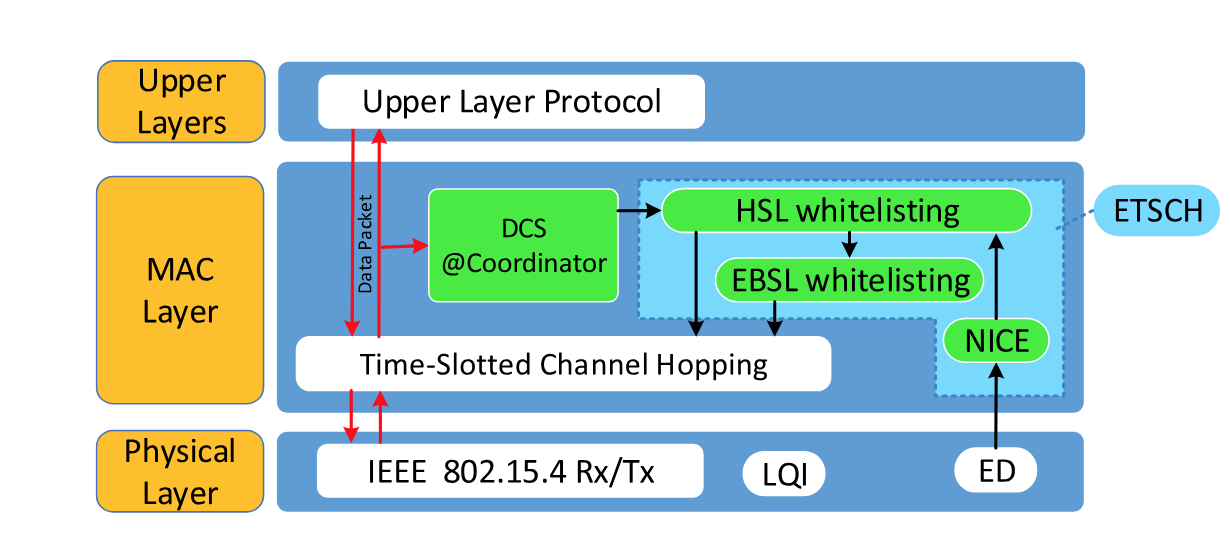
\includegraphics[height=6.5cm, width=\textwidth]{mac.png}
\caption{Coordinator Node Components}
\label{fig:lion}
\end{figure}

\end{frame}

\begin{frame}{Non-Intrusive Channel Quality Estimation (NICE)}
\begin{itemize}
  \item NICE provides centralized interference detection for ETSCH
  \\
  \item Problem: coordinator may cause interference for nodes
  \\
  \item Distributed channel quality sensing together with NICE
  \\
  \item  NICE cannot be used in other nodes to perform (Energy Detections) EDs and extract the quality of channels \cite{energy}
  \end{itemize}


\end{frame}

\begin{frame}{Algorithm}
\begin{itemize}
\end{itemize}
\begin{figure}[htp]
\centering
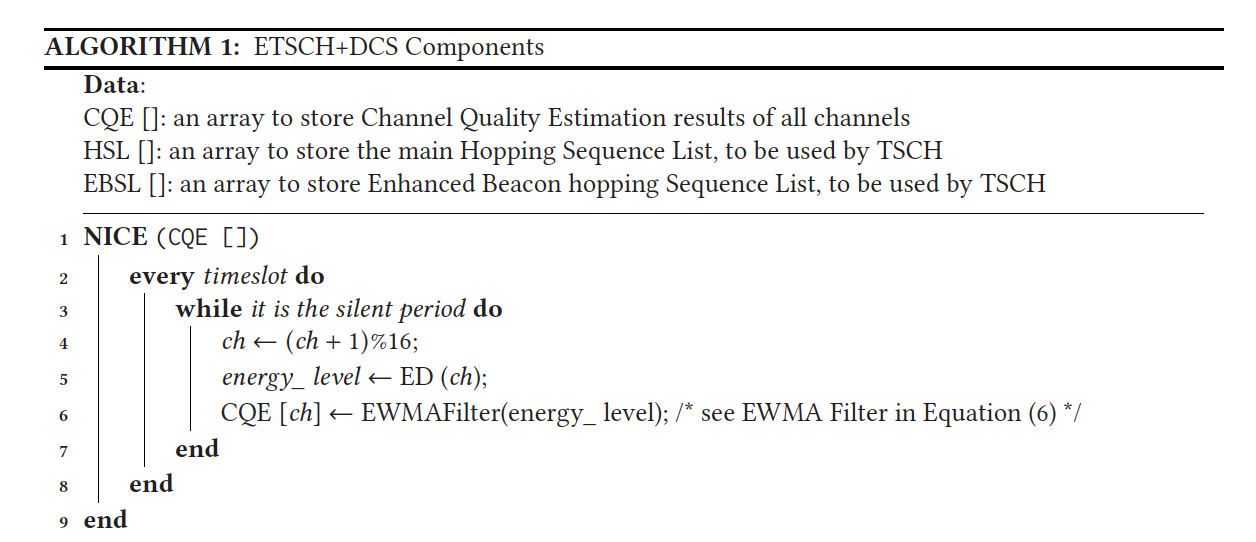
\includegraphics[height=6.5cm, width=\textwidth]{algo.png}
\label{fig:lion}
\end{figure}
\begin{itemize}
\end{itemize}

\end{frame}

\begin{frame}{Experiment}
\begin{itemize}
    \item{Noise Generators (NGs) detect noise interference on channels}
\end{itemize}
\begin{figure}[htp]
\centering
\vspace{-4mm}
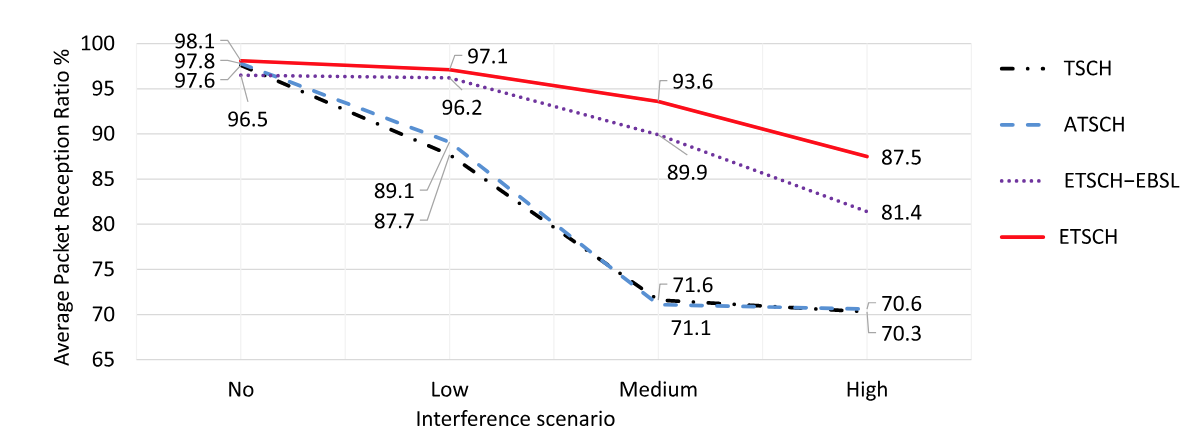
\includegraphics[height=6.1cm, width=\textwidth]{redgraph.png}
\label{fig:red}
\caption{Avg. PRR of Different Interference Scenarios}
\end{figure}
\end{frame}

\begin{frame}{Conclusions}
\begin{itemize}
  \item ETSCH and EBSL have higher PRR than plain TSCH and ATSCH.  
    \begin{itemize}
        \item less packet bursts/packet losses
    \end{itemize}
  \item NICE technique on its own isn't as effective
    \begin{itemize}
        \item DCS technique can detect and decrease existing interference
    \end{itemize}
\end{itemize}
\begin{itemize}
  \item Researching on, layering, and combining different protocols help improve the existing ones, thus mitigating interference, improving PRR, and improving the quality of the channels.  
\end{itemize}
\end{frame}

\begin{frame}{References}
\bibliographystyle{apalike} 
\bibliography{references} 
  \frametitle<presentation>{References}    
  \begin{thebibliography}{10}    
  \beamertemplatearticlebibitems
  \bibitem{wireless}
    Kannan Srinivasan, Maria A. Kazandjieva, Saatvik Agarwal, and Philip Levis.
    \newblock {\em The beta-factor-factor: Measuring
wireless link burstiness}.
    \newblock In Proceedings of the 6th ACM Conference on Embedded Network Sensor Systems (SenSys’08).
ACM, New York, NY, 29–42.
    
  \beamertemplatearticlebibitems
  \bibitem{energy}
    X. Vilajosana, Q. Wang, F. Chraim, T. Watteyne, T. Chang, and K. S. J. Pister.
    \newblock A realistic energy consumption
model for TSCH networks.
    \newblock IEEE Sens. J. 14, 2 (Feb. 2014), 482–489.
  \end{thebibliography}


\end{frame}



\end{document}

